\documentclass{article}

\usepackage{amsmath, amssymb, amsthm}
\usepackage[margin=0.6in]{geometry}
\usepackage[utf8]{inputenc}
\usepackage{hyperref}
\usepackage{graphicx}
\usepackage{pgf}
\graphicspath{{Images/}}
\DeclareUnicodeCharacter{2212}{-}

\hypersetup{
    colorlinks=true,
    urlcolor=blue,
}

\title{Forecasting Stock Price Using Sentiment Analysis and LSTM Networks}
\author{Blake Hillier, Grace Li, Joe Puhalla}
\date{May 11, 2020}

\begin{document}
\maketitle

\section{Overview}
Forecasting stock prices is a widely known problem many people have attempted to solve through various models. A common approach is to use only numerical data to predict tomorrow's price. However, investors often use the news about the company's decisions, the public's attitude towards the company, and the state of the economy when developing trading strategies. In this paper, we propose a model using macro-economic variables to predict the future price of a stock, one of which is statements from the Federal Reserve about decisions on economic policies. Our model is comprised of XLNet to perform sentiment analysis on one macro-economic variable and an LSTM Neural Network to combine all the variables while capturing the effect time has on the future stock price. In this paper we first explain the ideas behind XLNet and LSTM Neural Networks. We then explain our implementation of XLNet and LSTM and calculate their mean squared error (MSE) using appropriate subsets of our data. Finally, we explain how we use them together to forecast the stock price and calculate the entire models MSE before making some concluding remarks.

\section{XLNet}
XLNet is an autoregressive pretraining approach for NLP models. Pretraining a model is used to teach a model a broad field before being applied to a specific problem. This allows it to pick up potential nuances within the data and then apply this knowledge to better understand the specific problem. It also allows copies of the same model to be fine tuned to different problems, decreasing the total learning time. Autoregressive pretraining approaches create a conditional probability distribution based on the likelyhood function \begin{equation*}
    p(x)=\prod_{t=1}^{T}p(x_{t}|x_{<t})
\end{equation*} which only sees the relationship between previous text (it can also be modified to only see the relationship between text after the word). This is problematic since most words derive their meaning from context at both the beginning and the end of a sentence. XLNet solves this problem by calculating a distribution based on all the other text in the word by maximizing \begin{equation*}
    \max_{\theta}E_{z\sim Z_{T}}\left[\sum_{t=1}^{T}\log p_{\theta}(x_{z_{t}}|x_{z<t})\right]=E_{z\sim Z_{T}}\left[\sum_{t=1}^{T}\log\frac{e^{g_{\theta}(x_{z<t,z_{t}})l(x_{t}})}{\sum_{x^{'}}e^{g_{\theta}(x_{z<t,z_{t}})l(x^{'})}}\right]
\end{equation*} where $Z_{T}$ is the set of all permutations of text of length $T$, $z \in Z_{T}, x_{z<t}$ is the sequence of text from 1 to $t−1$, and $g_{\theta}$ transforms $x$ to a sequence of hidden words with the first $t-1$ set of words as additional information. They note the permutations don’t affect the actual order of the text sequence, just the factorization of the likelihood function. Because this is based on the likelihood function, it removes the idea each hidden text is independent of the others while still maintaining the benefits through encoding due to  $g_{\theta}$. In order for  $g_{\theta}$ to accomplish this, they split it into two different transforms: the query $g_{\theta}$ which looks at the first $t-1$ words in the permuted order to predict the  $t^{th}$ word, and the content  $h_{\theta}$ which simply encodes the first t words in the permuted order. The one downside to this model is the complexity of the optimization leading to a slower convergence. To reduce this problem, they adjust the equation to \begin{equation*}
    \max_{\theta}E_{z \sim Z_{T}}\left[\log_{p_{\theta}}(x_{z>c}|x_{z\leq t})\right]=E_{z\sim Z_{T}}\left[\sum_{t=c+1}^{|z|}\log p_{\theta}(x_{z_{t}}|x_{z<t})\right]
\end{equation*}
which changes the model to only predict the last $T - c$ words in the permutation order, where $c \approx \frac{T(1+K)}{K}$
for some parameter $K$.

\section{LSTM}

In this paper, the LSTM neural network is uesed to predict the stock price, the input data is the historical stock price and sentiment analysis results. Here, the sentiment based LSTM neural network (named sentiment-LSTM) is aimed to minimize the following loss function:

$$ \ell = min \sum_{t=p+1}^{p+T} \bigg\| X_{t} - \hat{X_{t}} \bigg\|_{2}^{2} $$

Where $T$ denotes the number of prediction time slots, i.e, $t$ = 1, ..., $p$ are the observations (training input data), $t = p+1, ..., p+T$ are the predicts (training output data); and $\hat{X}_{t}$ is given as following:

$$\hat{X}_t = \alpha X_{t}^{A} + \lambda S_{t}^{A} + c = \alpha X_{t}^{A} + \lambda f_{2}\underbrace{((S_{t-i})_{i=1}^{p})}_\text{Sentiment}+c$$

\begin{figure}[htp]
    \centering
    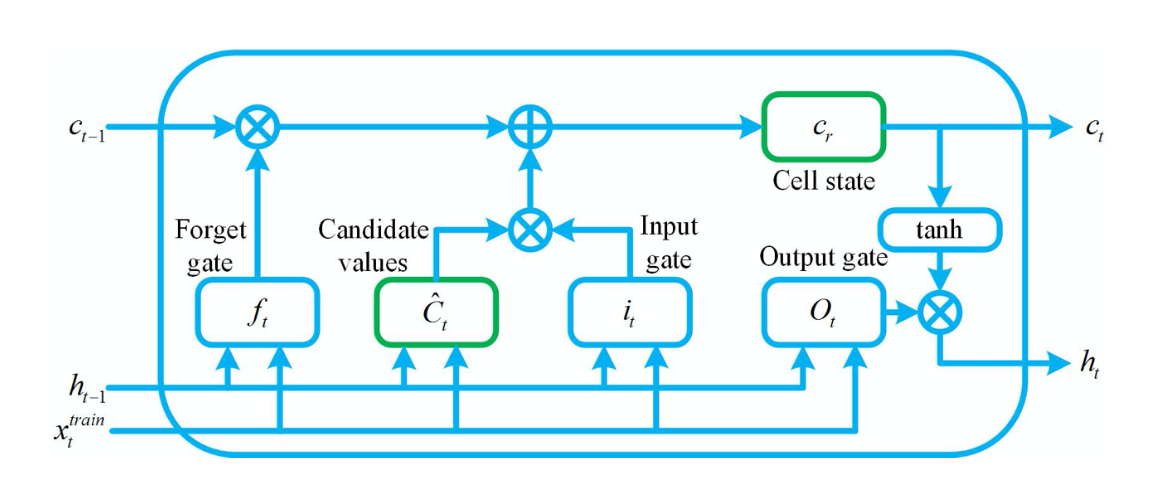
\includegraphics[width=7cm]{LSTM.png}
    \caption{LSTM Procedure}
    \label{fig:LSTM}
\end{figure}

Denote Formula as the training input data. Figure 1 shows the LSTM's structure network, which comprises one or more hidden layers, an output layer and an input layer. LSTM networks’ main advantage is that the hidden layer comprises memory cells. Each memory cell recurrently has a core self-connected linear unit called “ Constant Error Carousel, which provides short-term memory storage and has three gates:

\textbf{Input gate}, which controls the information from a new input to the memory cell, is given by

$$i_{t} = \sigma (W_{i} \times [h_{t-1}, \chi_{t}^{train}] + b_{i})$$
$$\hat{c_{t}} = tanh(W_{c} \times [h_{t-1}, \chi_{t}^{train}] + b_{c} )$$

$h_{t-1}$ is the hidden state at the time step $t-1;i_{t}$ is the output of the input gate layer at the time step $t; \hat{c_{t}} $ is the candidate value to be added to the output at the time step $t; b_{i}$ and $b_{c}$ are biases of the input gate layer and the candidate value computation, respectively; $W_{i}$ and $W_{c}$ are weights of the input gate and the candidate value computation respectively; and $\sigma (x) = 1/(1+e^{-x})$ is the pointwise nonlinear activation function.

\textbf{Forget gate}, which controls the limit up to which a value is saved in the memory, is given by
$$f(t) = \sigma (W_{f} \times [h_{t-1}, \chi_{t}^{train}]+b_{f})$$
where $f_{t}$ is the forget state at the time step $t, W_{f}$ is the weight of the forget gate; and $b_{f}$ is the bias of the forget gate.

\textbf{Output gate}, which controls the information output from the memory cell, is given by

$$ c_{t} = f_{t} \times c_{t-1} + i_{t} \times \hat{c_{t}}$$
$$o_{t} = \sigma (W_{o} \times [h_{t-1}, \chi_{t}^{train}] + b_{o})$$
$$h_{t} = o_{t} \times tanh(c_{t})$$

where new cell state $c_{t}$ are calculated based on the results of the previous two steps; $o_{t}$ is the output at the time step $t; W_{o}$ is the weight of the output gate; and $b_{o}$ is the bias of the out put gate. \\

\section{Experiment}
Because our model has multiple core algorithms, we need to calibrate each main component individually as well as when they are all together to ensure we are obtaining an optimal accuracy. This section will discuss the data we use, how each algorithm performs on their own, and how they perform when put together.
\subsection{Data}
Our data consisted of macroeconomic data and the FOMC Federal Statement text data. The macroeconomic data consisted of the quarterly GDP, monthly CPI, monthly unemployment rate, monthly inflation rate, the ten-year treasury rate, the 12-month LIBOR, and the FOMC statements from the Federal Reserve. All the data ranges from the beginning of the year 1994 to the end of 2019. We used Marathon Oil Corporation (MRO), Fifth Third Bancorp (FITB) and Devon Energy Corp (DVN) as stock data for algorithm training. Since our stock is daily data, all previous data were duplicated into daily data and aligned with the stock information. 

\subsection{Sentiment Analysis}
We used pytorch's implementation of XLNet-base for our model. Since we were analyzing statements from the fed, we felt the sentiment should come from a macro variable. If the variable increased to the next time-step, the sentiment was positive, and negative otherwise. Since we weren't sure which feature would work best with the stock, we decided to test GDP, Libor, Unemployment rates, and Inflation rates (MICH). We also tested a variety of batch sizes, maximum string lengths, and epochs to try and maximize the accuracy.
\begin{figure}[ht]
    \centering
    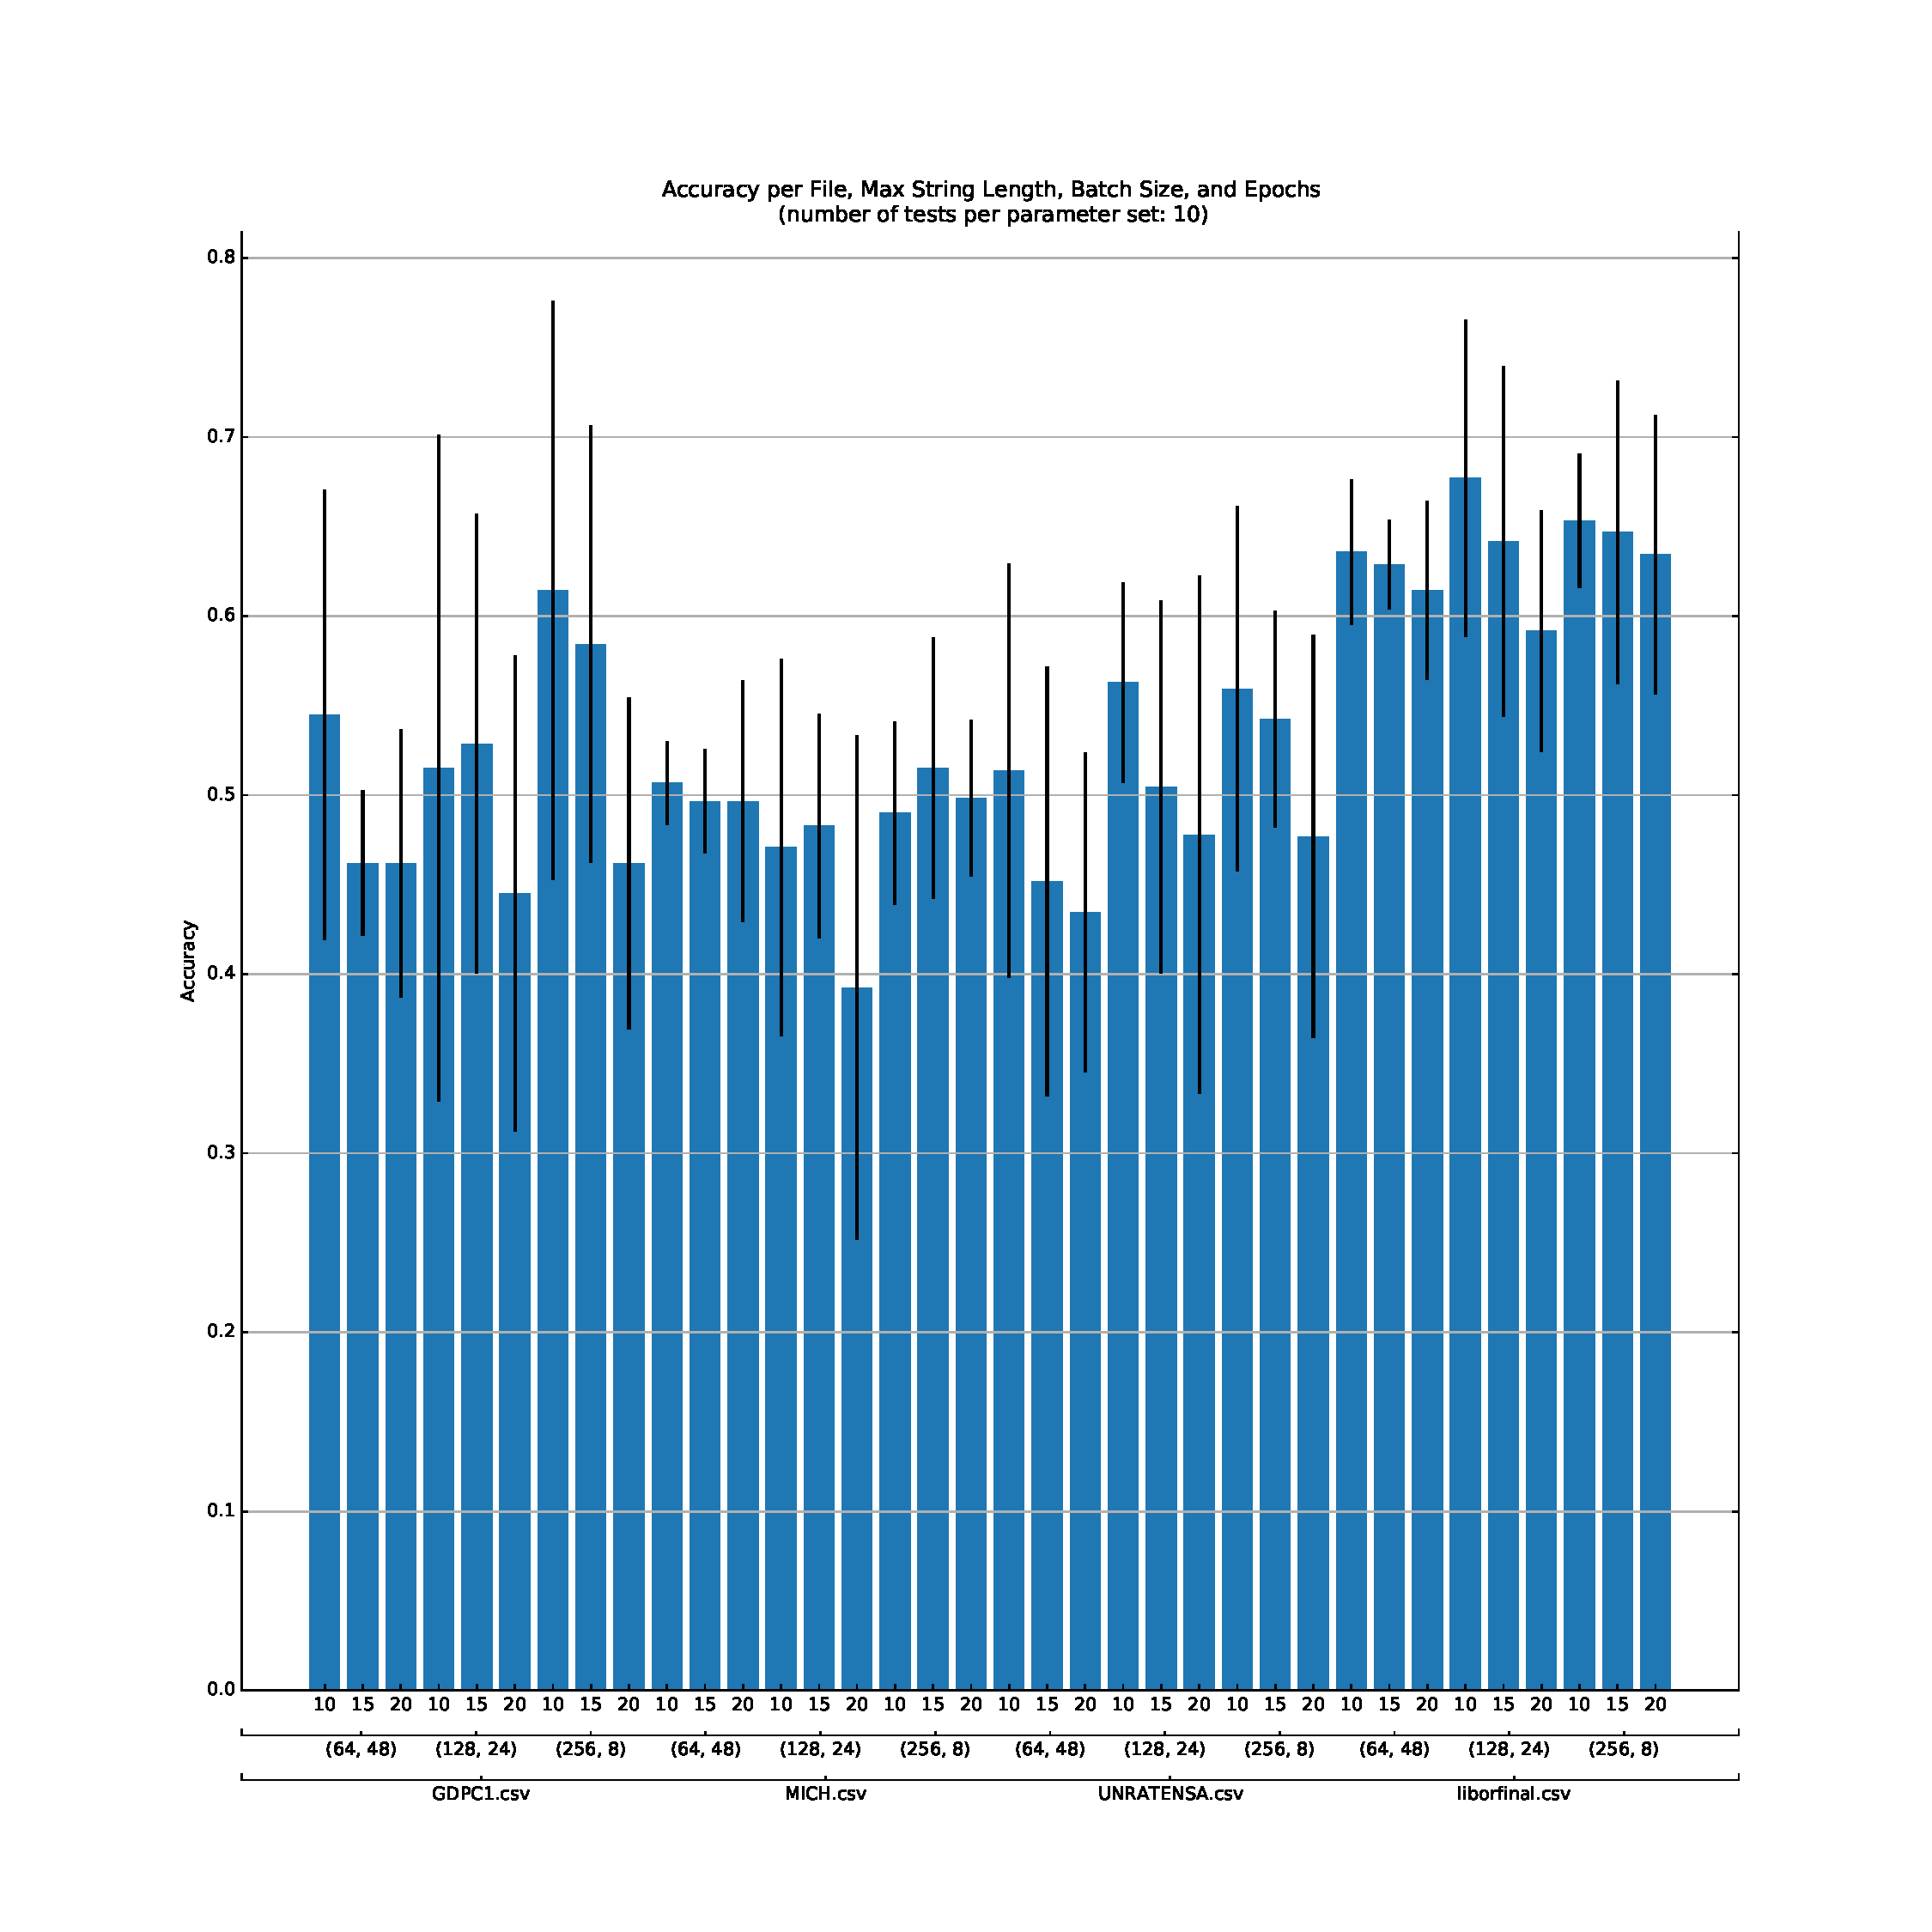
\includegraphics[width=1\textwidth]{Notes/ParameterSims3.pdf}
    \caption{Simulation results for XLNet parameter tests}
    \label{XLNParam}
\end{figure}
Figure $\ref{XLNParam}$ shows both the accuracy and the variance of the tests. Some results to note:
$$\begin{tabular}{c|c|c|c|c}
    Feature & String Length & Batch Size & Epochs & Accuracy \\ \hline
    GDP & 256 & 8 & 10 & 62\% \\
    MICH & 64 & 48 & 10 & 51\% \\
    UNEMP & 128 & 24 & 10 & 56\% \\
    Libor & 128 & 24 & 10 & 67\% \\
\end{tabular}$$
These parameter sets will be used to configure the final model when deciding which sentiment metric best helps forecast stock prices. 

\subsection{LSTM Stock Prediction}
\begin{figure}
\begin{minipage}{0.5\textwidth}
    \centering
    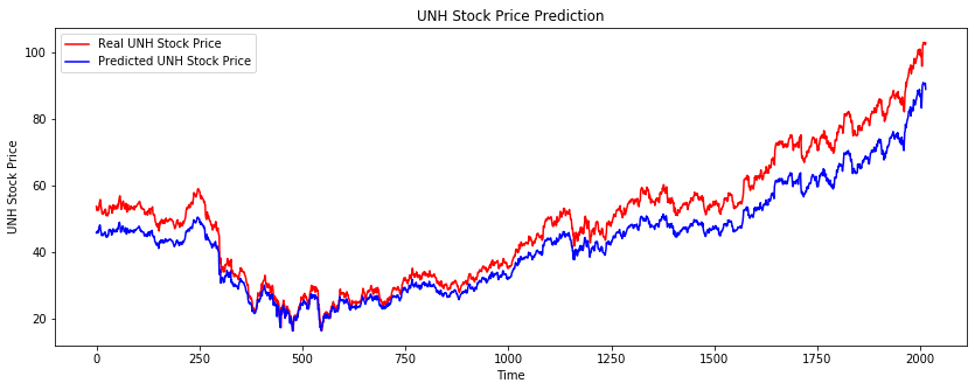
\includegraphics[width=9cm]{LSTMResult.png}
    \caption{Predicted vs. Actual Stock Price}
    \label{fig:LSTMForecast}
\end{minipage}
\begin{minipage}{0.5\textwidth}
    \centering
    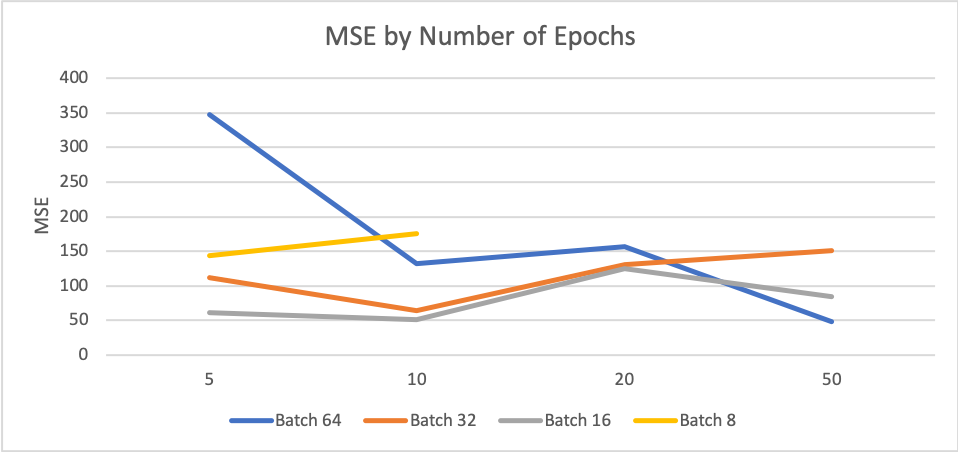
\includegraphics[width=9cm]{LSTMMSE.png}
    \caption{MSE by Number of Epochs}
    \label{fig:LSTMResult}
\end{minipage}
\end{figure}

The LSTM network we use includes four layers each with a dropout rate of twenty percent. The layers are of size $256,128,64,32$ and then the final layer. We sampled through several activation functions, starting with linear activation, and determined the ReLu activation to provide the best accuracy of the model. In order to determine the accuracy of the model, we plot both the predicted and actual stock price values. We then determine the mean squared error between the predicted and actual prices. We sample across several amounts of epochs and batch sizes in order to determine the best architecture for the model. For simplicity purposes, we used the already given ‘adam’ optimizer. With a batch size of 8, the 20 and 50 epoch sized networks caused memory issues and thus were unable to be completed. A batch size of 64, and 50 epochs yielded the lowest MSE among all models $(\ref{fig:LSTMForecast})$. Our feature set for the model were daily measures of price, GDP, CPI, inflation, unemployment, LIBOR, and the 10-year treasury yield. GDP data was given quarterly and thus had to be converted to daily data. In addition, CPI, inflation, and unemployment were given as monthly data and were converted to daily data. Our training data was from 1994 up to 2016 and our testing data was 2016 to 2019.
From out results for each stock we calculated the average mean squared error. The average mean squared error was 2559.10. Looking at each stock prediction, we observe that the LSTM model predicts some stocks very well, but also very poorly predicts a large amount of stocks. A selected group is shown in the appendix: FITB, DVN, and MRO.
\begin{figure}
    \centering
    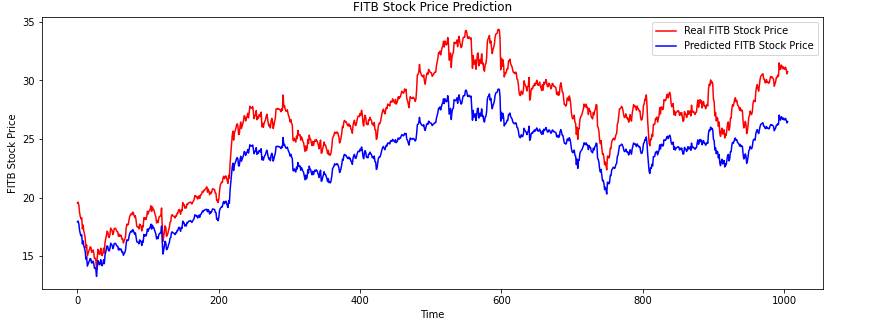
\includegraphics[width = 12cm]{Final FITB.png}
    \caption{LSTM Forecast compared with the actual price}
\end{figure}
\begin{figure}
    \centering
    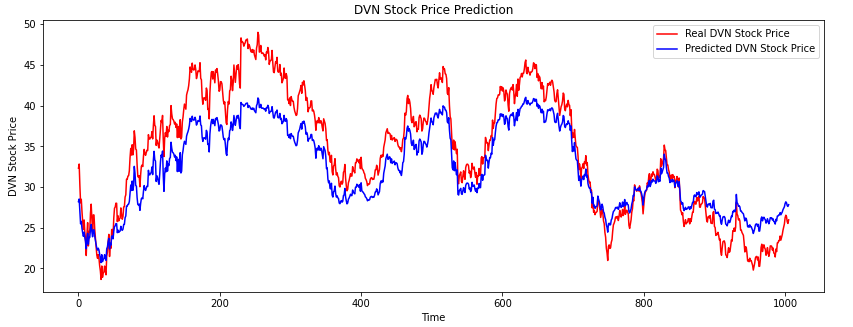
\includegraphics[width = 12cm]{Final DVN.png}
    \caption{LSTM Forecast compared with the actual price}
\end{figure}
\begin{figure}
    \centering
    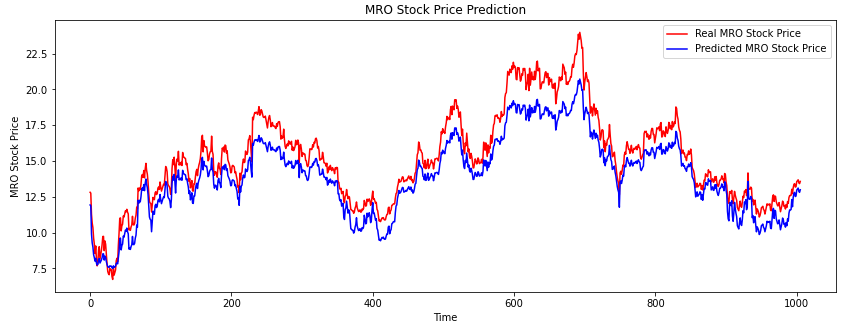
\includegraphics[width = 12cm]{Final MRO.png}
    \caption{LSTM Forecast compared with the actual price}
\end{figure}
There is a very high variance in the prediction power of our model. We also look at the distribution of the MSE scores for each stock in order to achieve a better understanding of the prediction power of our model. Looking at the distribution below for MSE values less than 500, we  see that most of the MSE values are in the range of 0 to 150.
\begin{figure}
    \centering
    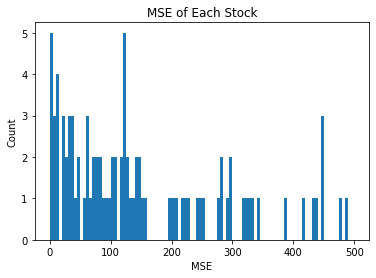
\includegraphics[width = 9cm]{MSE grouping.png}
    \caption{MSE Distribution}
\end{figure}
More tests need to be done to determine why some stocks are predicted incredibly well while others do so poorly so that we can reduce the variance of our model in the future. Increasing the the number of epochs might be able to reduce this variance at the expense of increasing computational time. Furthermore, the number of layers needs to be varied as well as the optimizer used. Tests need to be done to determine which features contribute the most to the predicting power of our model. Sentiment scores of the FOMC transcripts also need to be added as features of the model.  
\subsection{XLNet and LSTM}
After finding the most accurate sentiment prediction parameters and the best LSTM configuration, we tested both models working together. We first trained the XLNet on our calculated sentiment from a chosen macro feature. We then transformed all of the non-daily features into daily features, and began training the LSTM using our sentiment, macro features, and stock price for each stock. Lastly, we tested the model on the last four years of data to calculate it's MSE. We ran this experiment for each macro feature discussed in section 4.2 to see which feature helped create the most accurate predictions. Our results are below:
$$\begin{tabular}{c|c|c}
    Feature & Avg MSE & Variance \\ \hline
    GDP & 23704.33 & 64384386348.59  \\
    MICH & 35575.65 & 198994904967.61 \\
    UNEMP & 39754.39 & 198372093847.72\\
    Libor & 30592.24 & 125957788602.12 \\
\end{tabular}$$
We calculated the average MSE from each stock to judge the effectiveness of the macro feature, as well as the variance. Comparing this list to the one in 4.2, we see generally the more accurate XLNet is with a given macro feature, the better the combined model performs. Based on these tests, using GDP rates seems to be the best metric. Unfortunately, using XLNet did not improve the accuracy of the LSTM model. We can see some of the results from FITB, DVN, and MRO below.
\begin{figure}
    \centering
    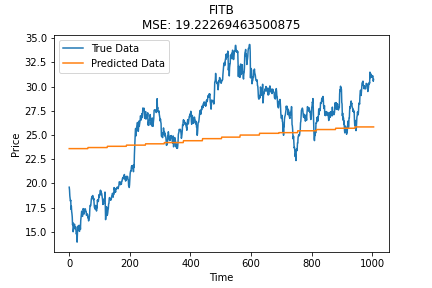
\includegraphics[]{Notes/FITBxln.png}
    \caption{Forecast with XLNet and LSTM compared with the actual price}
\end{figure}
\begin{figure}
    \centering
    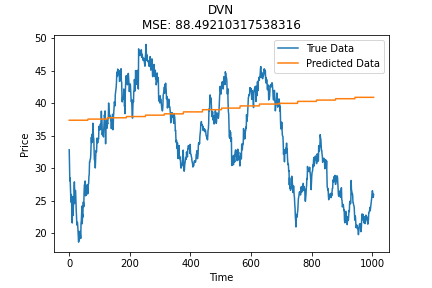
\includegraphics[]{Notes/DVNxln.png}
    \caption{Forecast with XLNet and LSTM compared with the actual price}
\end{figure}
\begin{figure}
    \centering
    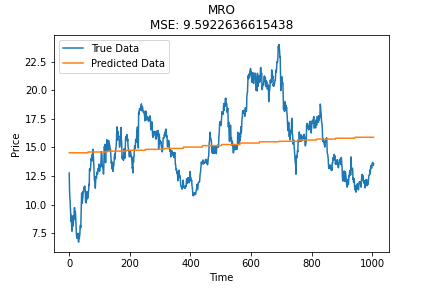
\includegraphics[]{Notes/MROxln.png}
    \caption{Forecast with XLNet and LSTM compared with the actual price}
\end{figure}

\section{Conclusion}
In this paper, we attempt to build a stock forecasting model using sentiment analysis with XLNet and then forecast using an LSTM network. Firstly, we used text data from Federal Reserve Statement because we considered the economic strategy Fed made can reflect the market's yearly performance. Secondly, we combined the XLNet sentiment analysis results with the LSTM to identify and extract opinions from the federal statements, combining the stock adjust the close price and macro-economic data to make stock prediction more accurate. However, the accuracy performance of XLNet-LSTM ends up with an MAE which is twice as much as the LSTM MAE. That means that XLNet can not make the prediction result more accurate and robust. Then we also used MSE as a loss function to further evaluate each feature. Among all the features we selected, LIBOR has the smallest MSE which means the LIBOR values dispersed closely to the central moment. Lastly, while judging the MSE of the predicted value is a great way of understanding the model's accuracy, simulating a trading strategy using the model would allow us to more concretely understand how usable our model really is. \par
While this project's results are disapointing, there are still things we can learn from this project. Looking back on this project, we think a few changes to our overall process would have resulted with a much better model. One is how we first approached this complex model. We should have spent more time configuring the LSTM before we began working on the XLNet in order to better optimize the predictive power of the LSTM model. Another problem is in how we combined the XLNet and the LSTM models. These should have been wired together to allow the error in the forecasts propagate back to the weights in XLNet. This would have also required us to create a unique loss function to evaluate the power of the sentiment from the XLNet as well. If this project was to be redone, these steps would either create a much more accurate model, or more firmly show this models inability to properly forecast a stocks price. For a full look at the code, check out our \href{https://github.com/BHill96/AdvancedBigDataAnalytics}{github}.

\begin{thebibliography}{9}
\bibitem{XLNet} 
Zhilin Yang, Zihang Dai, Yiming Yang, Jaime Carbonell, Ruslan Salakhutdinov, and Quoc V. Le. 
\textit{XLNet: Generalized Autoregresive Pretraining for Language Understanding}. 
Carnegie Mellon University, 2Google AI Brain Team, Jan $2^{nd}$ 2020.

\bibitem{LSTM} 
Xinyi Li, Yinchuan Li, Hongyang Yang, Liuqing Yang, Xiao-Yang Liu.
\textit{DP-LSTM: Differential Privacy-inspired LSTM for Stock Prediction Using Financial News}. Columbia University, Beijing Institute of Technology.

\bibitem{knuthwebsite} 
Github LSTM Stock Prediction,
\\\url{https://github.com/laxmimerit/Google-Stock-Price-Prediction-Using-RNN---LSTM/blob/master/Google%20Stock%20Price%20Prediction%20Using%20RNN-%20LSTM.ipynb}
\end{thebibliography}

\end{document}

